\documentclass[tikz,border=2pt]{standalone}
\usepackage{amsmath,amssymb}
\usepackage{pgfplots}
\pgfplotsset{compat=1.18}
\usetikzlibrary{arrows.meta}

\begin{document}
% a_n = 1/n -> 0. For epsilon = 0.1, every term with n >= N = 11 lies in the band (-0.1, 0.1)
% (a_10 = 0.1 is on the edge, not inside).
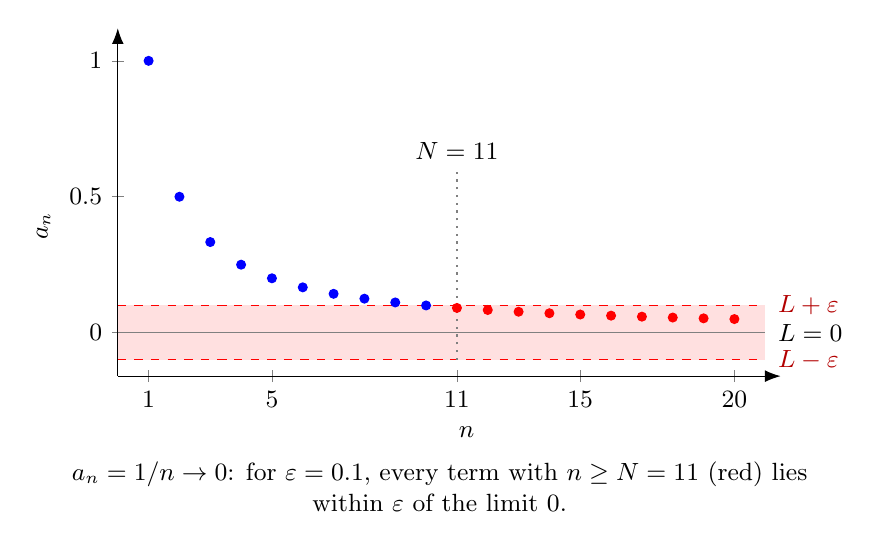
\begin{tikzpicture}[every node/.style={font=\small}]
	\begin{axis}[
		width=10cm, height=6cm,
		axis x line=bottom, axis y line=left, axis line style={-{Latex[length=2mm]}},
		xmin=0, xmax=21.5, ymin=-0.16, ymax=1.12,
		xtick={1,5,11,15,20}, ytick={0,0.5,1},
		tick label style={font=\small},
		xlabel={$n$}, ylabel={$a_n$},
		xlabel style={below right}, ylabel style={above left},
		clip=false
		]
		\fill[red!12] (axis cs:0,-0.1) rectangle (axis cs:21,0.1);
		\addplot[gray, domain=0:21] {0};
		\addplot[red, dashed, domain=0:21] {0.1};
		\addplot[red, dashed, domain=0:21] {-0.1};
		\addplot[gray, dotted, thick] coordinates {(11,-0.1) (11,0.6)};
		\addplot[only marks, mark=*, mark size=1.6pt, blue, samples at={1,...,10}] {1/x};
		\addplot[only marks, mark=*, mark size=1.6pt, red, samples at={11,...,20}] {1/x};
		\node[red!70!black, anchor=west, font=\small] at (axis cs:21.1,0.1) {$L+\varepsilon$};
		\node[anchor=west, font=\small] at (axis cs:21.1,0) {$L=0$};
		\node[red!70!black, anchor=west, font=\small] at (axis cs:21.1,-0.1) {$L-\varepsilon$};
		\node[anchor=south, font=\small] at (axis cs:11,0.6) {$N=11$};
	\end{axis}
	\node[anchor=north, align=flush center, text width=9.6cm] at ([yshift=-2pt]current bounding box.south) {$a_n=1/n\to0$: for $\varepsilon=0.1$, every term with $n\ge N=11$ (red) lies within $\varepsilon$ of the limit $0$.};
\end{tikzpicture}
\end{document}
